\section{Diffusion/mean square displacement}
\todod{Diffusion normal to and parallel to surface?}
\todob{Plot of $r^2$ for 200 and 40 states to argue for origo move?}

% bulk diff in Ref \#1 = 0.202034846318
%   N = mean(47577, 47524, 47555, 47552, 47559) = 
% bulk diff in Ref \#2 = 0.178684448075
%   N = mean(50280, 50284, 50291, 50275, 50321)

% bulk diff in Rough \#1 = 0.197721045372      
%   N = mean(4271, 4279, 4252, 4294, 4284)
% bulk diff in Rough \#2 = 0.208658027239  
%   N = mean(3414, 3396, 3419, 3431, 3393)


To produce these results we have averaged over 200 states, with 100 timesteps of 20.67 md units between each timestep ($\sim 0.5$ picoseconds\hl{???}), divided into 5 non-overlapping origos, with 40 states per origo.

We first look at the diffusion as function of distance to the silica matrix in the four reference systems, which we have plotted in \cref{fig:diffusion_reference_systems}. 
%
% \begin{figure}[htpb]%
%     \centering%
%     \includesvg[width=0.6\textwidth, svgpath=./images/diffusion/]{diffusion_constant_move_origin_reference01}%
%     \caption{%
%         Diffusion constant as function of distance to silica matrix for all four reference systems (flat fractures). The solid lines are for the two systems with 86 \AA\ wide fractures, and the dashed lines for narrow fractures of 14.4 and 28.8 \AA. \hl{FINISH CAPTION}. %
%         \label{fig:diffusion_reference_systems}%
%     }%
% \end{figure}%

We see that the diffusion constant has the similar quantitative behaviour as we move further from the silica matrix, but that the actual constant is different for each system. The four systems with 86 \AA\ wide fractures have diffusion constants that differ by around 10-30\%, even though those two systems should be pretty similar. The main difference between those two systems is the density, as we saw in \cref{sec:results_density}. We see the same thing for the bulk density, which is listed in \cref{tab:bulk_water_diffusion}, where reference system \#1 has a bulk diffusion constant of {0.202 \AA$^2$/ps}, while system \#2 has {0.179 \AA$^2$/ps}.

In \cref{fig:diffusion_rough_systems} we have plotted the diffusion constant as function of distance from the silica matrix for the four random fracture systems, ``rough \#1'' through 4. We again see a quantitative similar behaviour, and we see that all systems except the 14.4 \AA\ narrow fracture (``rough \#3'') have very similar diffusion constants. In \cref{tab:bulk_water_diffusion} see that the bulk diffusion constants in the two regular random fractures (\#1 and \#2) are similar, with a difference of $~6$\%, and close to the values at 8-10 \AA\ from the silica matrix in \cref{fig:diffusion_rough_systems}.
%
% \begin{figure}[htpb]%
%     \centering%
%     \includesvg[width=0.6\textwidth, svgpath=./images/diffusion/]{diffusion_constant_move_origin_rough01}%
%     \caption{%
%         Diffusion constant as function of distance to silica matrix for all four random/rough fractures. \hl{FINISH CAPTION}. %
%         \label{fig:diffusion_rough_systems}%
%     }%
% \end{figure}%
%
%
\begin{figure}[htpb]%
% \centering%
    \begin{minipage}[t]{0.499\textwidth}%
        \captionsetup{width=0.925\textwidth}%
        \centering%
        \includesvg[width=\textwidth, svgpath=./images/diffusion/]{diffusion_constant_move_origin_reference01}%
        \caption{%
            Diffusion constant as function of distance to silica matrix for all four reference systems (flat pores). The solid lines are for the two systems with 86 \AA\ wide pores, and the dashed lines for narrow fractures of 14.4 and 28.8 \AA. \hl{FINISH CAPTION}. %
%             \label{fig:diffusion_reference_systems}%
        }%
    \end{minipage}%
    \hfill%
    \begin{minipage}[t]{0.499\textwidth}% % change "b" to "t" to anchor top instead of bottom
        \captionsetup{width=0.925\textwidth}% % minipage defines a \textwidth for it's own, so we have to repeat this command inside the minipage
        \centering%
        \includesvg[width=\textwidth, svgpath=./images/diffusion/]{diffusion_constant_move_origin_rough01}%
        \caption{%
            Diffusion constant as function of distance to silica matrix for all four random rough fractures. Solid lines are for regular random fractures, and dashed lines for narrow fractures with uniform width of 14.4 and 28.8 \AA. \hl{FINISH CAPTION}. %
%             \label{fig:diffusion_rough_systems}%
        }%
    \end{minipage}%
\end{figure}%

% \begin{figure}[htpb]%
%     \centering%
%     {
%         \newcommand{\f}{\footnotesize}
%         \includesvg[width=0.7\textwidth, svgpath=./images/diffusion/]{diffusion01}%
%     }
%     \caption{%
%         Diffusion. \hl{Make new figure using new diffusion program}. %
% %         \label{fig:cell_lists}%
%     }%
% \end{figure}%

% \begin{figure}[htpb]%
%     \centering%
%     {
%         \newcommand{\f}{\footnotesize}%
%         \includesvg[width=0.7\textwidth, svgpath=./images/diffusion/]{diffusion_constant02}%
%     }
%     \caption{%
%         Diffusion. \hl{Make new figure using new diffusion program} \hl{FINISH CAPTION}. %
% %         \label{fig:cell_lists}%
%     }%
% \end{figure}%

%
\begin{table}[!htb]%
    \centering%
    \begin{tabular}{l|cc}%
        \textit{System} & Bulk $D$ [\AA$^2$/ps] & N    \\\hline
        Reference \#1   & 0.202                 & 48k  \\ % 0.202034846318
        Reference \#2   & 0.179                 & 50k  \\ % 0.178684448075
        Rough \#1       & 0.198                 & 4.3k \\ % 0.197721045372
        Rough \#2       & 0.209                 & 3.4k \\ % 0.208658027239
    \end{tabular}%
    \vspace{8pt}%
    \caption{%
        Bulk diffusion constant for water (for $r>10$ \AA), and the number of water molecules used in calculation. %
        \label{tab:bulk_water_diffusion}%
    }%
\end{table}

\begin{figure}[htpb]%
    \centering%
    \includesvg[width=0.8\textwidth, svgpath=./images/diffusion/]{diffusion_constant_move_origin_normal01}%
    \caption{%
        Diffusion for random rough fractures and reference systems. \hl{FINISH CAPTION}. %
%         \label{fig:cell_lists}%
    }%
\end{figure}%

\begin{figure}[htpb]%
    \centering%
    \includesvg[width=0.8\textwidth, svgpath=./images/diffusion/]{diffusion_constant_move_origin_narrow01}%
    \caption{%
        Diffusion for random narrow fractures and reference systems. \hl{FINISH CAPTION}. %
%         \label{fig:cell_lists}%
    }%
\end{figure}%

\begin{figure}[htpb]%
    \centering%
    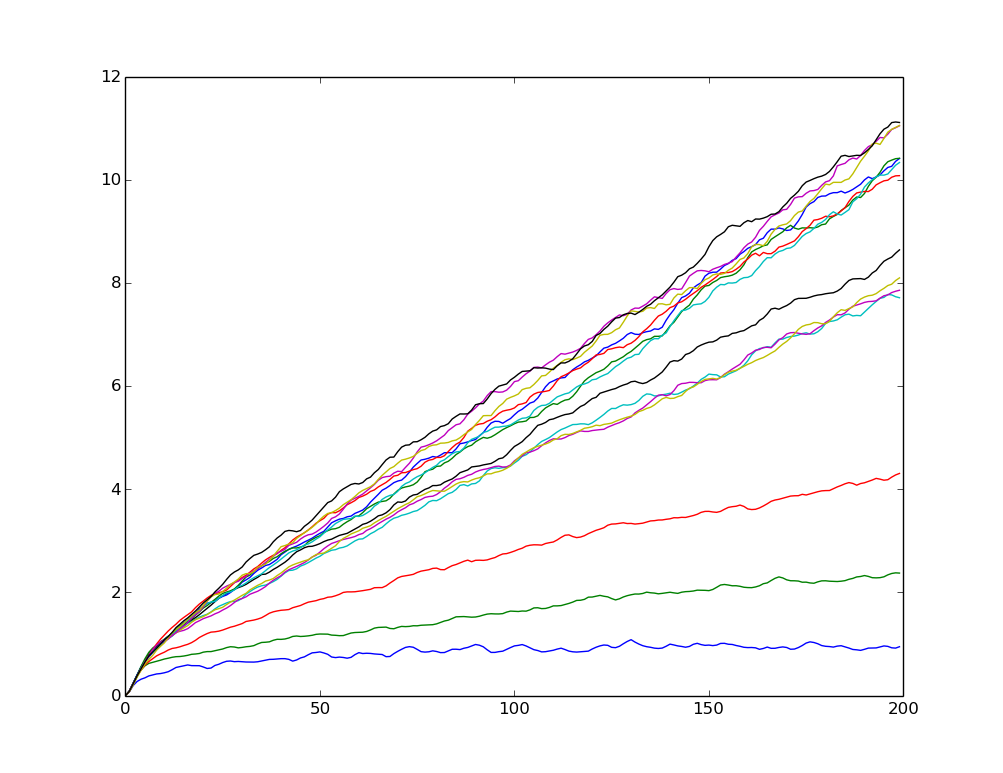
\includegraphics[width=0.5\textwidth]{images/diffusion/mean_square_displacement_interesting.png}%
    \caption{%
        Something interesting (msd stops increasing for a couple of angstrom near 4.5-5, 5-5.5, 5.5-6.0) \hl{FINISH CAPTION}. %
%         \label{fig:cell_lists}%
    }%
\end{figure}%

% \begin{figure}[htpb]%
%     \centering%
%     \setlength{\myfigwidth}{0.49\textwidth}%
% %     \setlength{\mycaptionwidth}{0.3\textwidth}%
% %
%     \begin{subfigure}[b]{\myfigwidth}%
%         \includesvg[width=\textwidth, svgpath=./images/diffusion/]{diffusion_constant_move_origin01}%
%         \caption{%
%             Diffusion. \hl{FINISH CAPTION}. %
%     %         \label{fig:cell_lists}%
%         }%
%     \end{subfigure}%
%     \hfill%
%     \begin{subfigure}[b]{\myfigwidth}%
%         \includesvg[width=\textwidth, svgpath=./images/diffusion/]{diffusion_constant_move_origin02}%
%         \caption{%
%             Diffusion. \hl{FINISH CAPTION}. %
%     %         \label{fig:cell_lists}%
%         }%
%     \end{subfigure}%
%     \caption{%
%         rough\_fracture\_01\_abel - ``Rough fracture \#1'' \hl{Caption} %
%         \label{fig:renderings_rough_fracture01_abel}%
%     }%
% \end{figure}%